\section{بخش چهارم: فیلتر \lr{Rank} و مقایسه زمان اجرا}

\begin{stepbox}
\field{هدف این بخش (بخش ۴)}{
جایگزینی عملگر \lr{Dilation} با فیلتر رتبه (\lr{Rank Filter}) مرتبه ۷ در ابعاد $51\times51$ به منظور بررسی بهبود مقاومت در برابر نویز، تکرار مراحل استخراج متن، و در نهایت مقایسه زمان اجرای محاسباتیِ این دو فیلتر.
}
\end{stepbox}

\subsection{کد پیاده‌سازی و اندازه‌گیری زمان}
از آنجا که فیلتر رتبه به صورت پیش‌فرض در توابع \lr{OpenCV} تعبیه نشده است، از کتابخانه \lr{SciPy} استفاده کرده و زمان اجرای هر دو فیلتر را برای مقایسه ثبت نمودیم:

\begin{codebox}[\lr{Rank Filter \& Execution Time}]
\begin{lstlisting}[language=Python]
import time
from scipy.ndimage import rank_filter

# Measure Dilation Time (for comparison)
start_time = time.time()
dilated = cv2.dilate(img, kernel_51, borderType=cv2.BORDER_CONSTANT, borderValue=0)
dilation_time = time.time() - start_time

# Measure Rank Filter Time (Rank 7 from top = -7 in Python)
start_time = time.time()
rank_img = rank_filter(img, rank=-7, size=(51, 51))
rank_time = time.time() - start_time

# The rest is the same subtraction and thresholding logic
diff_rank = cv2.subtract(rank_img, img)
ret, thresh_rank = cv2.threshold(diff_rank, 40, 255, cv2.THRESH_BINARY)
final_rank = cv2.bitwise_not(thresh_rank)
\end{lstlisting}
\end{codebox}

\newpage
\subsection{خروجی‌های تصویری}
تصاویر مربوط به خروجی فیلتر \lr{Rank}، تصویر تفاضل و استخراج نهایی متن در شکل \ref{fig:part4_rank} قابل مشاهده است.

\begin{figure}[h!]
    \centering
    \begin{subfigure}{0.31\textwidth}
        \centering
        
\includegraphics[width=\linewidth]{images/rank_51x51.jpg}
        \caption{پس‌زمینه (\lr{Rank})}
    \end{subfigure}
    \hfill
    \begin{subfigure}{0.31\textwidth}
        \centering
        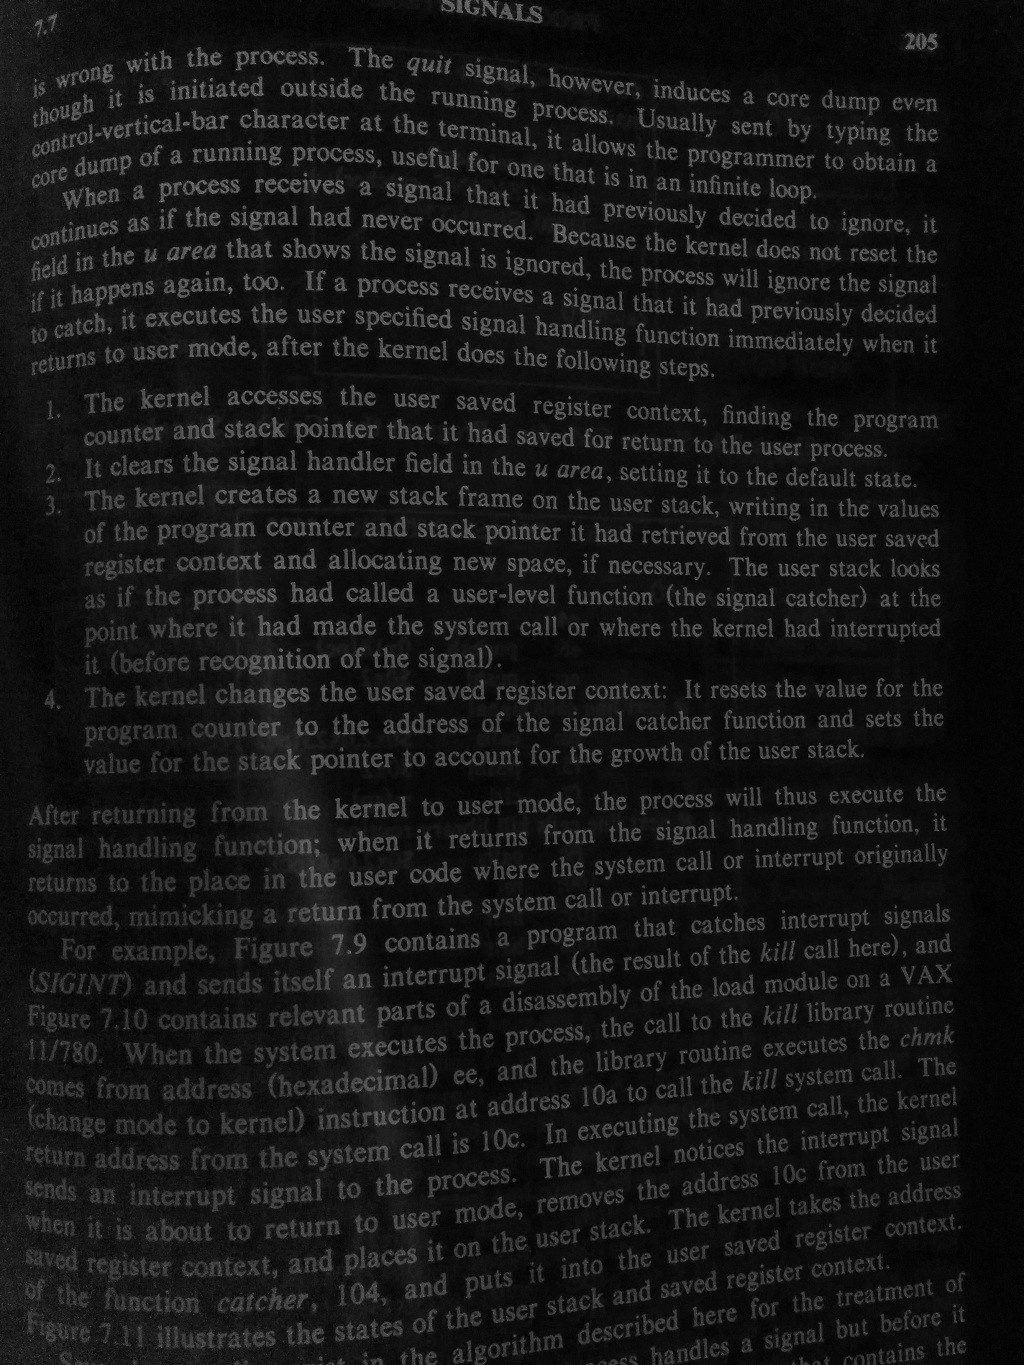
\includegraphics[width=\linewidth]{images/diff_rank_51x51.jpg}
        \caption{تفاضل (\lr{Rank})}
    \end{subfigure}
    \hfill
    \begin{subfigure}{0.31\textwidth}
        \centering
        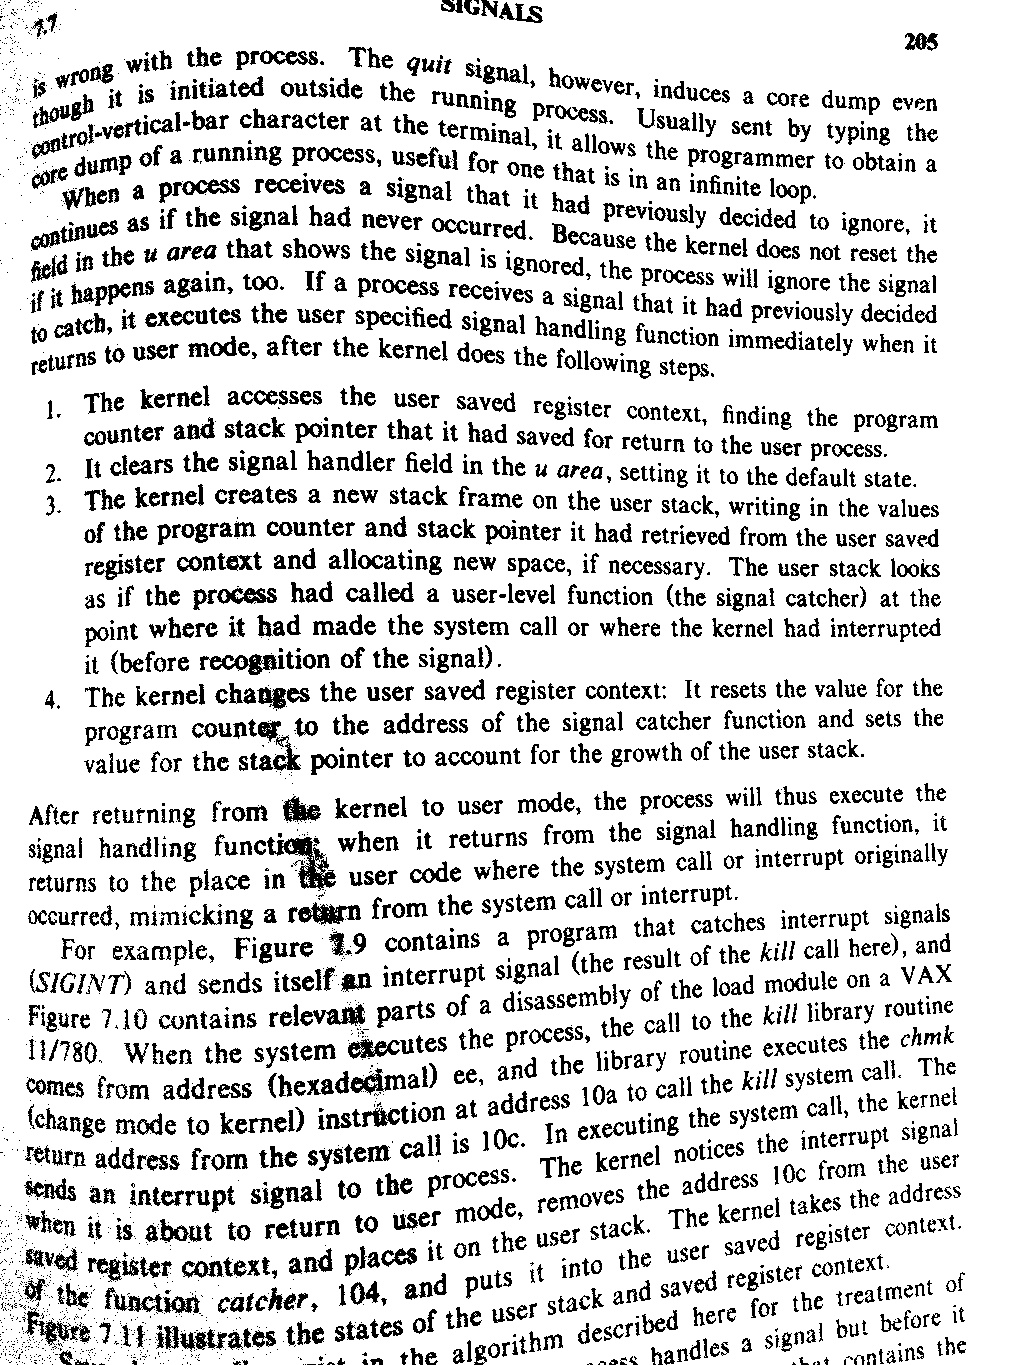
\includegraphics[width=\linewidth]{images/final_thresh_rank_51x51.jpg}
        \caption{نهایی (\lr{Rank})}
    \end{subfigure}
    \caption{مراحل استخراج متن با استفاده از فیلتر رتبه (\lr{Rank Filter})}
    \label{fig:part4_rank}
\end{figure}

\subsection{پاسخ به سوالات تمرین}
\textbf{آیا با استفاده از فیلتر \lr{Rank}، کیفیت نهایی بهبود یافته است؟} \\
فیلتر \lr{Rank} (رتبه ۷) به دلیل خاصیتِ نادیده گرفتنِ مقادیر حدی (\lr{Outliers})، مقاومت بهتری در برابر نویزهای نقطه‌ایِ روشنِ پس‌زمینه دارد. در واقع اگر نویزِ سفیدِ شدیدی در پس‌زمینه وجود داشت، \lr{Dilation} فریب می‌خورد اما \lr{Rank} از آن عبور می‌کرد و به صورت ساختاری، نقشه پس‌زمینه هموارتر و واقعی‌تری تولید می‌کرد. با این حال، در این تصویر خاصِ اسکن شده، چون نویز نقطه‌ای شدیدی در کاغذ نداریم، تفاوت کیفیتِ نهایی و تفکیک متن نسبت به \lr{Dilation} (با پنجره مشابه ۵۱) بسیار نامحسوس است.

\textbf{زمان اجرا فیلتر \lr{Rank} چقدر با عملگر \lr{Dilation} متفاوت است؟} \\
با توجه به خروجی‌های ثبت شده در هنگام اجرای کد:
\begin{itemize}
    \item \lr{Dilation Execution Time: 0.0020 seconds}
    \item \lr{Rank Filter Execution Time: 20.7522 seconds}
\end{itemize}
همان‌طور که اعداد نشان می‌دهند، عملگر \lr{Dilation} به شدت سریع‌تر (حدود ده هزار برابر سریع‌تر) اجرا می‌شود. دلیل این اختلافِ فاحش این است که \lr{OpenCV} برای \lr{Dilation} از الگوریتم‌های بسیار بهینه‌شده‌ای استفاده می‌کند که پیچیدگی زمانی آن‌ها کاملاً مستقل از ابعاد پنجره است ($O(1)$). اما فیلتر \lr{Rank} در هر بار حرکتِ پنجره روی تصویر، نیازمند ایجاد هیستوگرام محلی یا مرتب‌سازیِ مقادیرِ ۲۶۰۱ پیکسل (برای ابعاد ۵۱ در ۵۱) است که سربار محاسباتی فوق‌العاده بالایی به سیستم تحمیل می‌کند.